\chapter{Implementation strategies: evaluation and results}
\chaptermark{Implementation strategies: evaluation and results}
\label{chapter:exp_setup_results}
\minitoc

%%%%%%%%%%%%%%%%%%%%%%%%%%%%%%%%%%%%%%%%%%%%%%%%%%%%%%%%%%%%%%%%%%%%%%%%%%%%%%%%%%%%%%%%%%%%%%%
\section{Introduction}
The previous chapter presented two countermeasures against fault injection attacks and taking into account simple fault models, such as \textit{single-bit flip inside one register at a given clock cycle}. These countermeasures have been implemented by grouping the different DIFT-related registers in order to minimise the number of parity and redundancy bits. However, nowadays, studies~\cite{CGVCBLC-22-cardis,VDSPB-24-jce} have shown that is it possible to fault multiple bits precisely.

In this chapter, we present four different implementation's strategies of countermeasures to better protect the D-RI5CY mechanism against more complex fault models. Then, we evaluate each of these strategies in terms of security against more complex fault models. Finally, we compare them in terms of performance and area overhead. We implemented the minimisation of redundancy bits strategy in the last chapter. As shown in Chapter~\ref{chapter:countermeasures}, Hamming Code or even SECDED is better to use than just the simple parity for the correction and detection capacity. Hence, in this chapter, we do not implement others strategies for the simple parity protection. However, we present the results obtained from our simulations campaigns on the fault models considered in this chapter.

Section~\ref{section:chap6_faultmodels} introduces the different fault models considered.
Section~\ref{section:chap6_implem_strategies} introduces the four different strategies developed and assessed in this chapter.
Section~\ref{section:chap6_evaluation} presents the security assessment of these four strategies by giving the results associated to each fault model and the use cases to each strategy, and evaluate them in terms of security, performance, and area overhead.
Finally, in Section~\ref{section:chap6_discussion}, we discuss the results obtained from these five strategies according to their performance and area overhead and give the limitations for each strategy.

%%%%%%%%%%%%%%%%%%%%%%%%%%%%%%%%%%%%%%%%%%%%%%%%%%%%%%%%%%%%%%%%%%%%%%%%%%%%%%%%%%%%%%%%%%%%%%%
\section{Fault models considered in this chapter}
\label{section:chap6_faultmodels}
In Chapter~\ref{chapter:countermeasures}, we presented the results of fault injection campaigns targeting \textit{a single bit-flip in one register at a given clock cycle}, and \textit{a single bit-flip in two registers at two distinct clock cycles}. We demonstrated that lightweight countermeasures, such as simple parity, Hamming Code, or SECDED version of Hamming Code, are effective in protecting our DIFT mechanism against single bit-flips occurring in one register at one clock cycle or in two registers at two distinct clock cycles.

In this chapter, we extend our analysis to consider an attacker capable of injecting faults into DIFT-related registers, leading to a \textit{single bit-flip in two registers at a given clock cycle}. Furthermore, we account for an attacker able to induce \textit{multi-bit faults in one register at a given clock cycle}, as well as, \textit{multi-bit faults in two registers at a given clock cycle}. These fault models, introduced in Chapter~\ref{chapter:fissa}, are exhaustively tested across registers ranging from 1-bit to 10-bit. Registers larger than 10 bits, such as the configuration registers TPR and TCR, are excluded due to their size. For instance, simulating an exhaustive attack on a single 32-bit register for one cycle would require $2^{32}$ simulations (i.e: \powerTwo{pow(32,2)}{0} simulations), and for two 32-bit registers, the number of simulations would reach $2^{32} \times 2^{32}$ which is too large to be simulated in a reasonnable time. However, it is worth noting that the biggest register after these two 32-bit registers is a 6-bit register (cf. Tables~\ref{tab:strategies_register_info}, \ref{tab:sp_group}, \ref{tab:hammingcode_group}, \ref{tab:secded_group} \wip{mettre à jour avec tableaux ajouter dans partie évaluation}), so we fault every 1-bit to 6-bit registers.

The three fault models are exhaustively simulated across all possible values of these registers. To meet this objective, any DIFT-related register that maintains a 1-bit tag value, drives tag propagation or tag update processes, or holds security policy configurations, can be targeted. Additionally, registers storing redundancy bits for protection mechanisms are also considered.

% %%%%%%%%%%%%%%%%%%%%%%%%%%%%%%%%%%%%%%%%%%%%%%%%%%%%%%%%%%%%%%%%%%%%%%%%%%%%%%%%%%%%%%%%%%%%%%%
\section{Implementation strategies}
\label{section:chap6_implem_strategies}

Assessing the robustness of DIFT against more complex fault models requires comprehensive strategies that can identify vulnerabilities to enhance the system integrity. This section introduces four distinct strategies aimed at evaluating and enhancing the security of DIFT mechanisms against complex fault models. Each strategy offers a unique perspective on detecting, mitigating, or preventing the effects of multi bit-flip faults, contributing to a holistic approach in fortifying DIFT systems. By exploring these methodologies, we aim to provide actionable insights for developing more resilient DIFT solutions thanks to lightweight countermeasures.

\subsection{Strategy 2: Pipeline Stage Register Coupling for Robust Error Mitigation}

\begin{table}[t]
    \centering
    \footnotesize
    \caption{D-RI5CY Registers Details List for Strategy 2}
    \label{tab:strategy_2_register_info}
    % \setlength{\tabcolsep}{5pt}
    \begin{tabular}{@{}rccccccc@{}}
        \toprule
        Register Name                   & Module                                & Size   & \tableTwoLines{Strategy}{2} \\\midrule
        pc\_id\_o\_tag                  & \textcolor{red}{Instruction}          & 1      & Gr1                         \\
        pc\_if\_o\_tag                  & \textcolor{red}{Fetch Stage}          & 1      & Gr1                         \\\hdashline
        alu\_operand\_a\_ex\_o\_tag     &                                       & 1      & Gr2                         \\
        alu\_operand\_b\_ex\_o\_tag     &                                       & 1      & Gr2                         \\
        alu\_operand\_c\_ex\_o\_tag     &                                       & 1      & Gr2                         \\
        alu\_operator\_o\_mode          &                                       & 2      & Gr2                         \\
        check\_d\_o\_tag                &                                       & 1      & Gr2                         \\
        check\_s1\_o\_tag               &                                       & 1      & Gr2                         \\
        check\_s2\_o\_tag               & \textcolor{blue}{Instruction}         & 1      & Gr2                         \\
        is\_store\_post\_o\_tag         & \textcolor{blue}{Decode Stage}        & 1      & Gr2                         \\
        memory\_set\_o\_tag             &                                       & 1      & Gr2                         \\
        regfile\_alu\_waddr\_ex\_o\_tag &                                       & 5      & Gr2                         \\
        register\_set\_o\_tag           &                                       & 1      & Gr2                         \\
        store\_dest\_addr\_ex\_o\_tag   &                                       & 1      & Gr2                         \\
        store\_source\_ex\_o\_tag       &                                       & 1      & Gr2                         \\
        use\_store\_ops\_ex\_o          &                                       & 1      & Gr2                         \\\hdashline
        rf\_reg[0]                      &                                       & 1      & Gr3                         \\
        rf\_reg[1]                      &                                       & 1      & Gr3                         \\
        rf\_reg[2]                      & \textcolor{LimeGreen}{Register File}  & 1      & Gr3                         \\
        \ldots                          & \textcolor{LimeGreen}{Tag}            & \ldots & Gr3                         \\
        rf\_reg[30]                     &                                       & 1      & Gr3                         \\
        rf\_reg[31]                     &                                       & 1      & Gr3                         \\\hdashline
        rs1\_o\_tag                     & \textcolor{DarkOrange}{Execute Stage} & 1      & Gr4                         \\\hdashline
        tcr\_q                          & \textcolor{DarkRed}{Control and}      & 32     & Gr5                         \\
        tpr\_q                          & \textcolor{DarkRed}{Status Registers} & 32     & Gr6                         \\\hdashline
        data\_type\_q\_tag              &                                       & 2      & Gr7                         \\
        data\_we\_q\_tag                & \textcolor{magenta}{Load/Store}       & 1      & Gr7                         \\
        rdata\_offset\_q\_tag           & \textcolor{magenta}{Unit}             & 2      & Gr7                         \\
        rdata\_q\_tag                   &                                       & 4      & Gr7                         \\
        \bottomrule
    \end{tabular}
\end{table}

\begin{table}[t]
    \centering
    \footnotesize
    \caption{DIFT-related protected registers -- Strategy 2}
    \label{tab:strategy_2_groups}
    \begin{tabular}{@{}rccccc@{}}
        \toprule
                & Protected stage          & \tableTwoLines{Number of}{bits} & \tableTwoLines{Number of}{protected bits} & \tableTwoLines{Number of}{redundancy bits} & \tableTwoLines{Number of}{parity bits} \\ \midrule
        Group 1 & Instruction Fetch Stage  &                                 &                                           &                                            &                                        \\
        Group 2 & Instruction Decode Stage &                                 &                                           &                                            &                                        \\
        Group 3 & Register File Tag        &                                 &                                           &                                            &                                        \\
        Group 4 & Execute Stage            &                                 &                                           &                                            &                                        \\
        Group 5 & TCR                      &                                 &                                           &                                            &                                        \\
        Group 6 & TPR                      &                                 &                                           &                                            &                                        \\
        Group 7 & Load/Store Unit          &                                 &                                           &                                            &                                        \\ \midrule
        Total   &                          &                                 &                                           &                                            &                                        \\
        \bottomrule
    \end{tabular}
\end{table}

\subsection{Strategy 3: Individual Register Encapsulation for Fault Tolerance}

\subsection{Strategy 4: DIFT-Enhanced CSR Register Slicing for Strengthened Security}

\subsection{Strategy 5: Sliced Register Bit Coupling for Improved Data Integrity}

\begin{figure}[ht]
    \centering
    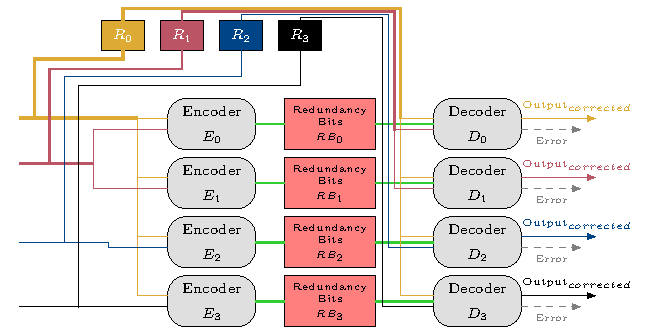
\includegraphics[page=1]{c6_group_composition/img/implem5_spaghetti.pdf}
    \caption{Strategy 5 -- Implementation idea}
    \label{fig:strategy_5_functionning}
\end{figure}

%%%%%%%%%%%%%%%%%%%%%%%%%%%%%%%%%%%%%%%%%%%%%%%%%%%%%%%%%%%%%%%%%%%%%%%%%%%%%%%%%%%%%%%%%%%%%%%
\section{Experimental results}
\label{section:chap6_evaluation}

\begin{table}[t]
    \centering
    \footnotesize
    \caption{D-RI5CY Registers Details List}
    \label{tab:strategies_register_info}
    \setlength{\tabcolsep}{5pt}
    \begin{tabular}{@{}rccccccc@{}}
        \toprule
        Register Name                   & Module                                & Size   & \tableTwoLines{Strategy}{1} & \tableTwoLines{Strategy}{2} & \tableTwoLines{Strategy}{3} & \tableTwoLines{Strategy}{4} & \tableTwoLines{Strategy}{5} \\
        \midrule
        pc\_id\_o\_tag                  & \textcolor{red}{Instruction}          & 1      & Gr5                         & Gr1                            &                             &                             &                             \\
        pc\_if\_o\_tag                  & \textcolor{red}{Fetch Stage}          & 1      & Gr5                         & Gr1                            &                             &                             &                             \\\hdashline
        alu\_operand\_a\_ex\_o\_tag     &                                       & 1      & Gr5                         & Gr2                            &                             &                             &                             \\
        alu\_operand\_b\_ex\_o\_tag     &                                       & 1      & Gr5                         & Gr2                            &                             &                             &                             \\
        alu\_operand\_c\_ex\_o\_tag     &                                       & 1      & Gr5                         & Gr2                            &                             &                             &                             \\
        alu\_operator\_o\_mode          &                                       & 2      & Gr5                         & Gr2                            &                             &                             &                             \\
        check\_d\_o\_tag                &                                       & 1      & Gr5                         & Gr2                            &                             &                             &                             \\
        check\_s1\_o\_tag               &                                       & 1      & Gr5                         & Gr2                            &                             &                             &                             \\
        check\_s2\_o\_tag               & \textcolor{blue}{Instruction}         & 1      & Gr5                         & Gr2                            &                             &                             &                             \\
        is\_store\_post\_o\_tag         & \textcolor{blue}{Decode Stage}        & 1      & Gr5                         & Gr2                            &                             &                             &                             \\
        memory\_set\_o\_tag             &                                       & 1      & Gr5                         & Gr2                            &                             &                             &                             \\
        regfile\_alu\_waddr\_ex\_o\_tag &                                       & 5      & Gr4                         & Gr2                            &                             &                             &                             \\
        register\_set\_o\_tag           &                                       & 1      & Gr5                         & Gr2                            &                             &                             &                             \\
        store\_dest\_addr\_ex\_o\_tag   &                                       & 1      & Gr5                         & Gr2                            &                             &                             &                             \\
        store\_source\_ex\_o\_tag       &                                       & 1      & Gr5                         & Gr2                            &                             &                             &                             \\
        use\_store\_ops\_ex\_o          &                                       & 1      & Gr5                         & Gr2                            &                             &                             &                             \\\hdashline
        rf\_reg[0]                      &                                       & 1      & Gr3                         & Gr3                            &                             &                             &                             \\
        rf\_reg[1]                      &                                       & 1      & Gr3                         & Gr3                            &                             &                             &                             \\
        rf\_reg[2]                      & \textcolor{LimeGreen}{Register File}  & 1      & Gr3                         & Gr3                            &                             &                             &                             \\
        \ldots                          & \textcolor{LimeGreen}{Tag}            & \ldots & Gr3                         & Gr3                            &                             &                             &                             \\
        rf\_reg[30]                     &                                       & 1      & Gr3                         & Gr3                            &                             &                             &                             \\
        rf\_reg[31]                     &                                       & 1      & Gr3                         & Gr3                            &                             &                             &                             \\\hdashline
        rs1\_o\_tag                     & \textcolor{DarkOrange}{Execute Stage} & 1      & Gr5                         & Gr4                            &                             &                             &                             \\\hdashline
        tcr\_q                          & \textcolor{DarkRed}{Control and}      & 32     & Gr1                         & Gr5                            &                             &                             &                             \\
        tpr\_q                          & \textcolor{DarkRed}{Status Registers} & 32     & Gr2                         & Gr6                            &                             &                             &                             \\\hdashline
        data\_type\_q\_tag              &                                       & 2      & Gr5                         & Gr7                            &                             &                             &                             \\
        data\_we\_q\_tag                & \textcolor{magenta}{Load/Store}       & 1      & Gr5                         & Gr7                            &                             &                             &                             \\
        rdata\_offset\_q\_tag           & \textcolor{magenta}{Unit}             & 2      & Gr5                         & Gr7                            &                             &                             &                             \\
        rdata\_q\_tag                   &                                       & 4      & Gr5                         & Gr7                            &                             &                             &                             \\
        \bottomrule
    \end{tabular}
\end{table}


\begin{table}[t]
    \centering
    \footnotesize
    \caption{Registers by Strategy: Summary of Number and Size}
    \label{tab:strategies_summary}
    \begin{tabular}{rcc}
        \toprule
        Strategy                 & Number of Registers & Number of Bits \\
        \midrule
        Baseline -- D-RI5CY      & 55                  & 127            \\
        Strategy Simple Parity 1 & 60                  & 132            \\
        Strategy Hamming code 1  & 60                  & 152            \\
        Strategy Hamming code 2  & 62                  & 157            \\
        Strategy Hamming code 3  & 79                  & 191            \\
        Strategy Hamming code 4  & 93                  & 228            \\
        Strategy Hamming code 5  & 94                  & 241            \\
        Strategy SECDED code 1   & 65                  & 157            \\
        Strategy SECDED code 2   & 69                  & 164            \\
        Strategy SECDED code 3   & 103                 & 215            \\
        Strategy SECDED code 4   & 131                 & 266            \\
        Strategy SECDED code 5   & 133                 & 280            \\
        \bottomrule
    \end{tabular}
\end{table}


%%%%%%%%%%%%%%%%%%%%%%%%%%%%%%%%%%%%%%%%%%%%%%%%%%%%%%%%%%%%%%%%%%%%%%%%%%%%%%%%%%%%%%%%%%%%%%%
\section{Discussion}
\label{section:chap6_discussion}

%%%%%%%%%%%%%%%%%%%%%%%%%%%%%%%%%%%%%%%%%%%%%%%%%%%%%%%%%%%%%%%%%%%%%%%%%%%%%%%%%%%%%%%%%%%%%%%
\section{Summary}


%%%%%%%%%%%%%%%%%%%%%%%%%%%%%%%%%%%%%%%%%%%%%%%%%%%%%%%%%%%%%%%%%%%%%%%%%%%%%%%%%%%%%%%%%%%%%%%